
\chapter{Link and Star Technique}\label{chap4}

\section{Abstract Theory I}\pageoriginale\label{chap4-sec4.1}

\begin{definition}[Join of open simplexes]\label{chap4-defi4.1.1}
Suppose $\sigma$ and two open simplexes in the same vector space. We say that $\sigma\tau$ {\em is defined}, when
\begin{itemize}
\item[(a)] the sets of vertices of $\sigma$ and $\tau$ are disjoint

\item[(b)] the union of the set of vertices of $\sigma$ and $\tau$ is independent.
\end{itemize}
\end{definition}

In such a case we define $\sigma\tau$ to be the open simplex whose set of vertices is the union of those of $\sigma$ and of $\tau$. If $\sigma$ is a $0$-simplex, we will denote $\sigma\tau$ by $\{x\}\tau$ or $\tau\{x\}$ where $x$ is the unique point in $\sigma$.

We also, by convention, where $\sigma$ (or $\tau$) is taken to be the empty set $\emptyset$, make the definition
$$
\emptyset\sigma=\sigma\emptyset=\sigma
$$

Clearly $\dim \sigma\tau=\dim \sigma+\dim\tau+1$, even when one or both of them are empty.

\begin{ex}\label{chap4-ex4.1.2}
$\sigma \tau$ is defined if and only if $\overline{\sigma}\cap \overline{\tau}=\emptyset$, and any two open intervals $O(x,y)$, $O(x',y')$ are disjoint, where $x$, $x'\in\overline{\sigma}$, $y$, $y'\in \overline{\tau}$, $x\neq x'$ or $y\neq y'$. In this case $\sigma\tau$ is the union of open $1$-simplexes $O(x,y)$, $x\in \sigma$, $y\in \tau$.
\end{ex}

This is easy. Actually it is enough to assume $O(x,y)\cap O(x',y')=\emptyset$ for $x$, $x'\in\sigma$, $y$, $y'\in\tau$; $x\neq x'$ or $y\neq y'$. That\pageoriginale it is true for points of $\overline{\sigma}$ and $\overline{\tau}$ and $\overline{\sigma}\cap \overline{\tau}=\emptyset$ follow from this.

\begin{ex}\label{chap4-ex4.1.3}
When $\sigma\tau$ is defined, the faces of $\sigma \tau$ are the same as $\sigma'\tau'$, where $\sigma'$ and $\tau'$ are faces of $\sigma$ and $\tau$ respectively. If either $\sigma'\neq \sigma$ or $\tau'\neq \tau$, then $\sigma'\tau'$ is a proper face of $\sigma\tau$.
\end{ex}

\begin{ex}\label{chap4-ex4.1.4}
Let $\sigma$ and $\tau$ be in ambient vector spaces $V$ and $W$. In $V\times W\times \mathbb{R}$, let $\widetilde{\sigma}=\sigma\times 0\times 0$ and $\overline{\tau}=0\times \tau\times 1$. Then $\widetilde{\sigma}\widetilde{\tau}$ is defined. 
\end{ex}

\begin{definition}\label{chap4-defi4.1.5}
Let $\mathscr{S}$ be a simplicial presentation, and $\sigma$ an element of $\mathscr{S}$. Then the {\em link of $\sigma$ in} $\mathscr{S}$ denoted by $Lk(\sigma,\mathscr{S})$ is defined as
\begin{align*}
& Lk(\sigma,\mathscr{S})=\left\{\tau \in\mathscr{S}|\sigma\tau\quad\text{is defined.}\right\}\\
Lk(\sigma,\mathscr{A})=\mathscr{S}\quad \text{if}\quad \sigma=\emptyset.
\end{align*}

Obviously $Lk(\sigma,\mathscr{S})$ is a subpresentation of $\mathscr{S}$. 

In case $\sigma$ is $0$-dimensional, we write $Lk(x,\mathscr{S})$ for $Lk(\sigma,\mathscr{S})$ where $x$ is the unique element in $\sigma$.
\end{definition}

\begin{ex}\label{chap4-ex4.1.6}
If $\tau\in Lk(\sigma,\mathscr{S})$, then
$$
Lk(\tau, Lk(\sigma,\mathscr{S}))=Lk(\sigma\tau,\mathscr{S}).
$$
\end{ex}

\begin{notation}\label{chap4-not4.1.7}
If $\sigma$ is an open simplex, then $\{\overline{\sigma}\}$ and $\{\partial \sigma\}$ will denote the simplicial presentations of $\overline{\sigma}$ and $\p \sigma$ made up of faces of $\sigma$.
\end{notation}

\begin{ex}\label{chap4-ex4.1.8}
If $\tau=\rho\sigma$, and $\dim \rho\geq 0$, then
\begin{align*}
& Lk(\rho,\{\p \tau\})=\{\p \sigma\}\\
& Lk(\rho,\{\overline{\tau}\})=\{\overline{\sigma}\}.
\end{align*}
\end{ex}

\begin{definition}\label{chap4-defi4.1.9}
Let\pageoriginale $\mathfrak{a}$ and $\mathscr{B}$ be simplicial presentations such that for all $\sigma\in \mathfrak{a}$, $\tau\in\mathscr{B}$, $\sigma\tau$ is defined, and $\sigma\tau\cap \sigma'\tau'=\emptyset$ if $\sigma\neq \sigma'$ or $\tau\neq \tau'$. Then we say that the {\em join of} $\mathfrak{a}$ and $\mathscr{B}$ {\em is defined}, and define the {\em join of $\mathfrak{a}$ and $\mathscr{B}$}, denoted by $\mathfrak{a}\ast\mathscr{B}$ to be the set
$$
\left\{
\begin{array}{r}
\sigma\tau|\sigma\in\mathfrak{a},\ \tau\in \mathscr{B}\ \sigma\text{~ or~ }\tau~ \text{ may be empty}\\
\text{but not both.\ }
\end{array}
\right\}
$$

By \ref{chap4-ex4.1.3} $\mathfrak{a}\ast \mathscr{B}$ is a simplicial presentation. If $\emptyset$ is empty, we define $\mathfrak{a}\ast\phi=\phi\ast\mathfrak{a}=\mathfrak{a}$.
\end{definition}

In case $\mathfrak{a}$ and $\mathscr{B}$ are presentations of polyhedra in $V$ and $W$, then we construct, by \ref{chap4-ex4.1.4}, $\widetilde{\mathfrak{a}}$ and $\widetilde{\mathscr{B}}$ which are isomorphic to $\mathfrak{a}$ and $\mathscr{B}$, and for which we can define $\widetilde{\mathfrak{a}}\ast\widetilde{\mathscr{B}}$. It clearly depends only on $\mathfrak{a}$ and $\mathscr{B}$ upto simplicial isomorphism; in this way we can construct {\em abstractly} any joins we desire. 

\begin{ex}\label{chap4-ex4.1.10}
$\mathfrak{a}\ast\mathscr{B}=\mathscr{B}\ast\mathfrak{a}$

$\mathfrak{a}\ast(\mathscr{B}\ast\mathscr{C})=(\mathfrak{a}\ast\mathscr{B})\ast\mathscr{C}$. 

That is whenever one side is defined, the other also is defined and both are equal. 
\end{ex}

\begin{ex}\label{chap4-ex4.1.11}
If $\alpha\in\mathfrak{a}$, $\beta\in\mathscr{B}$, then
$$
Lk(\alpha\beta,\mathfrak{a}\ast\mathscr{B})=Lk(\alpha,\mathfrak{a})\ast Lk(\beta,\mathscr{B}). 
$$

In particular, when $\beta=\emptyset$,
$$
Lk(\alpha,\mathfrak{a}\ast\mathscr{B})=Lk(\alpha,\mathfrak{a})\ast\mathscr{B}
$$
and when $\mathscr{L}=\emptyset$,
$$
Lk(\beta,\mathfrak{a}\ast\mathscr{B})=\mathfrak{a}\ast Lk(\beta,\mathscr{B}).
$$
\end{ex}

If $\mathfrak{a}$ is the presentation of a single point $\{v\}$, and is joinable to $\mathscr{B}$, then we call $\mathfrak{a}\ast\mathscr{B}$; the {\em cone} on $\mathscr{B}$ with {\em vertex} $v$,\pageoriginale and denote it by $C(\mathscr{B})$. $\mathscr{B}$ is called the {\em base} of the cone. If we make the convention, that the unique regular presentation of a one point polyhedron $v$, is to be written $\{\{v\}\}$, then $C(\mathscr{B})=\{\{v\}\}\ast\mathscr{B}$.

\begin{definition}\label{chap4-defi4.1.12}
Let $\mathscr{S}$ be a simplicial presentation, and $\sigma\in \mathscr{S}$. Then the {\em star of $\sigma$ in $\mathscr{S}$}, denoted by $St(\sigma,\mathscr{S})$, is defined to be $\{\overline{\sigma}\}\ast Lk(\sigma,\mathscr{S})$.
\end{definition}

Clearly $St(\sigma,\mathscr{S})$ is a subpresentation of $\mathscr{S}$ and is equal to $\cup \{\{\overline{\tau}\}|\tau\in\mathscr{S},\sigma\leq \tau\}$.

In case $\sigma$ contains only a single point $x$, we write $St(x,\mathscr{S})$.

\begin{ex}\label{chap4-ex4.1.13}
Let $\mathscr{S}$ be a simplicial presentation, $\sigma$ an element of $\mathscr{S}$. If $\tau$ is a face of $\sigma$ with $\dim \tau=\dim\sigma-1$, then
$$
Lk(\sigma,\mathscr{S})=Lk(\tau,\{\partial\sigma\}\ast Lk(\sigma,\mathscr{S})).
$$
\end{ex}

\begin{definition}\label{chap4-defi4.1.14}
If $\mathscr{S}$ is a simplicial presentation, the $k$-skeleton of $\mathscr{S}$, denoted by $\mathscr{S}_{k}$ is defined to be
$$
\mathscr{S}_{k}=\cup \{\{\overline{\sigma}\}|\sigma\in\mathscr{S}\dim \sigma\leq k\}.
$$
\end{definition}

Clearly $\mathscr{S}_{k}$ is a subpresentation of $\mathscr{S}$.

\begin{ex}\label{chap4-ex4.1.15}
If $\sigma\in \mathscr{S}_{k}$ and $\dim \sigma=\ell$, $(\ell\leq k)$, then
$$
Lk(\sigma,\mathscr{S}_{k})=Lk(\sigma,\mathscr{S})_{k-\ell-1}.
$$
\end{ex}

\begin{ex}\label{chap4-ex4.1.16}
Let $f:P\to Q$ be a polyhedral map, simplicial with respect to presentations $\mathscr{S}$ and $\mathscr{S}'$ of $P$ and $Q$ respectively. Then
\begin{itemize}
\item[(1)] $f(\mathscr{S}_{k})\subset (\mathscr{S}'_{k})$

\item[(2)] If $\sigma\in \mathscr{S}$, $f(St(\sigma,\mathscr{S}))\subset St(f\sigma,\mathscr{S}')$

\item[(3)] For\pageoriginale every $\sigma\in \mathscr{S}$, $f(Lk(\sigma,\mathscr{S}))\subset Lk(f(\sigma),\mathscr{S}')$ if and only if $f$ maps every $1$-simplex of $\mathscr{S}$ onto a $1$-simplex of $\mathscr{S}'$.
\end{itemize}
\end{ex}

(Strictly speaking, these are the maps induced by $f$).

\section{Abstract Theory II}\label{chap4-sec4.2}

\begin{definition}\label{chap4-defi4.2.1}
Let $\mathscr{P}$ be a regular presentation and $\eta$ a centering of $\mathscr{P}$. Let $A\in \mathscr{P}$. Then {\em the dual of $A$} and the {\em link of $A$, with respect of $\eta$}, denoted by $\delta A$ and $\lambda A$ are defined to be 
\begin{align*}
& \delta A=\left\{0(\eta C_{0},\ldots,\eta C_{k})\mid A\leq C_{0}<\ldots<C_{k},k\geq 0\right\}\\
& \lambda A=\left\{0(\eta C_{0},\ldots,\eta C_{k})\mid A<C_{0}<\ldots<C_{k},k\geq 0\right\}
\end{align*}
where $C_{i}\in\mathscr{P}$ for all $i$.
\end{definition}

Clearly $\delta A$ and $\lambda A$ are subpresentations of $d\mathscr{P}=d(\mathscr{P},\eta)$. When there are several regular presentations to be considered, we will denote these by $\delta_{\mathscr{P}}A$ and $\lambda_{\mathscr{P}}A$. $\eta$ will be usually omitted from the terminology, and these will be simply called {\em dual of} $A$ and {\em link of $A$.}

\setcounter{subsection}{1}
\subsection{}\label{chap4-sec4.2.2}
Every simplex of $d\mathscr{P}$ belongs to some $\delta A$.

\subsection{}\label{chap4-sec4.2.3}
$\delta A$ is the cone on $\lambda A$ with vertex $\eta A$.

\setcounter{proposition}{3}
\begin{ex}\label{chap4-ex4.2.4}
Let $\dim A=p$, and consider any $p$-simplex $\sigma$ of $d\mathscr{P}$ contained in $A$ i.e. $\sigma=0(\eta B_{0},\ldots, \eta B_{p})$, for some $B_{0}<\ldots<B_{p}=A$. Then $\lambda A=Lk(\sigma,d\mathscr{P})$.
\end{ex}

\setcounter{subsection}{4}
\subsection{}\label{chap4-sec4.2.5}
Suppose $\mathscr{P}$ is, in fact, simplicial. Then we have defined both $\lambda A$ and $Lk(A,\mathscr{P})$. These are related thus:

A\pageoriginale vertex of $\lambda A$ is of the form $\eta C$ where $A<C$. There is a unique $B$ of $\mathscr{P}$ such that $C=AB$. $\eta B$ is a typical vertex of $d(Lk(A,\mathscr{P}))$. The correspondence $\eta C\leftrightarrow \eta B$ defines a simplicial isomorphism:
$$
\lambda A\leftrightarrow d(Lk(A,\mathscr{P})).
$$

\setcounter{proposition}{5}
\begin{ex}\label{chap4-ex4.2.6}
With the notation of \ref{chap4-defi4.2.1}, $A<B$ if and only if $\delta B\subset \lambda A$. For any $A\in \mathscr{P}$, $\lambda A$ is the union of all $\delta B$ for $A<B$.
\end{ex}

\begin{ex}\label{chap4-ex4.2.7}
If $\mathscr{P}$ is {\em simplicial}, $A$, $B\in\mathscr{P}$, then $\delta A\cap \delta B\neq \emptyset$ if and only if $A$ and $B$ are faces of a simplex of $\mathscr{P}$. If $C$ is the minimal simplex of $\mathscr{P}$ containing both $A$ and $B$ (that $C$ is the open simplex generated by the union of the vertices of $A$ and $B$), then $\delta A\cap \delta B=\delta C$.
\end{ex}

\begin{definition}\label{chap4-defi4.2.8}
If $\mathscr{P}$ is a regular presentation and $\eta$ a centering of $\mathscr{P}$, {\em the dual $k$-skeleton of $\mathscr{P}$}, denoted by $\mathscr{P}^{k}$ is defined to be
$$
\mathscr{P}^{k}=
\left\{
\begin{array}{rr}
0(\eta C_{0},\ldots,\eta C_{p})\mid C_{0}<\ldots<C_{p},\dim C_{0}\geq k,\\
p\geq 0,\quad C_{i}\in \mathscr{P}.\qquad
\end{array}
\right\}
$$
\end{definition}

Clearly $\mathscr{P}^{k}$ is a subpresentation of $d\mathscr{P}$, and is, in fact the union of all $\delta A$ for $\dim A\geq k$. It is even the union of all $\delta A$ for $\dim A=k$.

Thus $\delta A$, $\lambda A$, $\mathscr{P}^{k}$ are all simplicial presentations. 

\begin{ex}\label{chap4-ex4.2.9}
$d\mathscr{P}=\mathscr{P}^{0}\supset \mathscr{P}'\supset \ldots \supset \mathscr{P}^{n}\supset \mathscr{P}^{n+1}=\emptyset$, where $n$ is the dimension of $\mathscr{P}$. Dim $\mathscr{P}^{k}=n-k$.
\end{ex}

We shall be content with the computation of links of vertices of $\mathscr{P}^{k}$. 

\begin{ex}\label{chap4-ex4.2.10}
If\pageoriginale $A\in\mathscr{P}$, $\dim A\geq k$, then
$$
Lk(\eta A,\mathscr{P}^{k})=\{\partial A\}^{k}\ast \lambda A.
$$
\end{ex}

Next, we consider the behaviour of polyhedral maps with respect to duals.

Let $f:P\to Q$ be a polyhedral map; let $\mathscr{P}$ and $\mathcal{Q}$ be two simplicial presentations of $P$ and $Q$ respectively with respect to which $f$ is simplicial. If $\mathscr{V}$ is a centering of $\mathcal{Q}$, it can be {\em lifted} to a centering $\eta$ of $\mathscr{P}$, that is $f(\eta A)=\mathscr{V}f(A)$ for all $A\in \mathscr{P}$. (see \ref{chap2-sec2.2}). $f$ is simplicial with respect to $d(\mathscr{P},\eta)$ and $d(\mathcal{Q},\mathscr{V})$ also. Now,

\setcounter{subsection}{10}
\subsection{}\label{chap4-sec4.2.11}
If $A\in \mathscr{P}$, $f(\delta_{\mathscr{P}}A)\subset \delta_{\mathcal{Q}}(f(A))$. 

\subsection{}\label{chap4-sec4.2.12}
If $B\in \mathcal{Q}$, then $f^{-1}(\delta_{\mathcal{Q}}B)=\cup \{\delta_{\mathscr{P}}A|f(A)=B\}$. 

\begin{remark*}
All these should be read as maps induced by $f$, etc. Since each such $A$ must have dimension $\geq \dim B$, we have
\end{remark*}

\setcounter{proposition}{12}
\begin{proposition}\label{chap4-prop4.2.13}
With the above notation, for each $k$, $f^{-1}(\mathcal{Q}^{k})\subset \mathscr{P}^{k}$.
\end{proposition}

This property is dual to the property with respect to the usual skeleta ``$f(\mathscr{P}_{k})\subset \mathcal{Q}_{k}$''.

\begin{corollary}\label{chap4-coro4.2.14}
If $\dim P=n$, then $\dim f^{-1}(\mathcal{Q}^{k})\leq n-k$.
\end{corollary}

In particular, if $\dim Q=m$, and $q$ is a point of an (open)
$\mathfrak{m}$ - dimensional simplex of $\mathcal{Q}$, $f^{-1}(q)$ is $a\leq (n-m)$-dimensional subpolyhedron of $P$.

\begin{ex}\label{chap4-ex4.2.15}
$f^{-1}(\mathcal{Q}')=\mathscr{P}^{1}$, if and only if every $1$-simplex of $\mathscr{P}$ is mapped onto a $1$-simplex of $\mathcal{Q}$. (i.e. no $1$-simplex of $\mathscr{P}$ is collapsed to a simple point).
\end{ex}

\section{Geometric Theory}\pageoriginale\label{chap4-sec4.3}

\begin{definition}\label{chap4-defi4.3.1}
Let $P$ and $Q$ be polyhedra in the same vector space $V$. We say that the {\em join of $P$ and $Q$ is defined} (or $\underline{P\ast Q}$ {\em is defined}, of {\em $P$ and $Q$ are joinable}), if:
\begin{itemize}
\item[(a)] $P\cap Q=\emptyset$

\item[(b)] If $x$, $x'\in P$, $y$, $y'\in Q$, and either $x\neq x'$ or $y\neq y'$; then $O(x,y)\cap O(x',y')\neq \emptyset$. 
\end{itemize}

If the join of $P$ and $Q$ is defined, we define the {\em join} of $P$ and $Q$, denoted by $P\ast Q$ to be
$$
P\ast Q=\cup \left\{x,y]\mid x\in P, y\in Q\right\}
$$
\end{definition}

By definition, $P\ast\emptyset=\emptyset\ast P=P$.

Every point $z\in P\ast Q$ can be written as:
$$
z=(1-t)x+ty,\quad x\in P,\quad y\in Q,\quad 0\leq t\leq 1.
$$

The number $t$ is uniquely determined by $z$; $y$ is uniquely determined if $z\not\in P$ (i.e.\@ if $t\neq 0$), $x$ is uniquely determined if $z\not\in Q$ (i.e.\@ if $t\neq 1$).

\setcounter{subsection}{1}
\subsection{}\label{chap4-sec4.3.2}
Let $\mathscr{P}$ and $\mathcal{Q}$ be simplicial presentations of $P$ and $Q$; and suppose the (geometric) join $P\ast Q$ is defined. Then by \ref{chap4-ex4.1.2}, the (simplicial) join $\mathscr{P}\ast \mathcal{Q}$ is defined, and we have $|\mathscr{P}\ast\mathcal{Q}|=P\ast Q$.

This shows that $P\ast Q$ is a polyhedron.

\setcounter{proposition}{2}
\begin{definition}\label{chap4-defi4.3.3}
If $P_{1}$, $Q_{1}$, $P_{2}$, $Q_{2}$ are polyhedra such that $P_{1}\ast Q_{1}$ and $P_{2}\ast Q_{2}$ are defined, and $f:P_{1}\to P_{2}$, $g:Q_{1}\to Q_{2}$ are maps, {\em then the join of $f$ and $g$}, denoted by $f\ast g$, is the map from $P_{1}\ast Q_{1}$ to $P_{2}\ast Q_{2}$ given by,
$$
(f\ast g)((1-t)x+ty)=(1-t)f(x)+tg(y)
$$
$x\in P_{1}$, $y\in Q_{1}$, $0\leq t\leq 1$.
\end{definition}

\setcounter{subsection}{3}
\subsection{}\label{chap4-sec4.3.4}
In\pageoriginale the above if $f: \mathcal{P}_{1}\to \mathcal{P}_{2}$, $g:\mathcal{Q}_{1}\to \mathcal{Q}_{2}$ are simplicial with respect to $\mathscr{P}_{1}$, $\mathscr{P}_{2}$; $\mathcal{Q}$, $\mathcal{Q}_{2}$, then $f\ast g:P_{1}\ast Q_{1}\to P_{2}\ast Q_{2}$ is simplicial with respect to $\mathscr{P}_{1}\ast\mathcal{Q}_{1}$ and $\mathscr{P}_{2}\ast\mathcal{Q}_{2}$. Thus the join of polyhedral maps is polyhedral.


\subsection{}\label{chap4-sec4.3.5}
If $P\ast Q$ is defined, $(\Id)_{p}\ast(\Id_{Q})=\Id_{P\ast Q}$. If, $P_{1}\ast Q_{1}$, $P_{2}\ast Q_{2}$, $P_{3}\ast Q_{3}$ are defined and $f_{1}:P_{1}\to P_{2}$, $f_{2}:P_{2}\to P_{3}$, $g_{1}:Q_{1}\to Q_{2}$, $g_{2}:Q_{2}\to Q_{3}$ are maps, then
$$
(f_{2}\circ f_{1})\ast (g_{2}\circ g_{1})=(f_{2}\ast g_{2})\circ (f_{1}\ast g_{1})
$$

This says that the join is a functor of two variables from pairs of polyhedra for which join is defined and pairs of polyhedral maps, to polyhedra and polyhedral maps.

The join of a polyhedron $P$ and a single point $v$ is called the {\em cone} on $P$, (sometimes denoted by $C(P)$) with {\em base} $P$ and vertex $v$.

\setcounter{proposition}{5}
\begin{ex}\label{chap4-ex4.3.6}
$C(P)$ is contractible.
\end{ex}

\begin{ex}\label{chap4-ex4.3.7}
$P\ast Q-Q$ contains $P$ as a deformation retract.
\end{ex}

\noindent
{\bf Hint:}~Use the map given by $(*)$ below.

Let us suppose that $P\ast Q$ and the cone $C(Q)$ with vertex $v$ are both defined. The interval $[0,1]$ is $0*1$, and so two maps can be defined:
\begin{align*}
&\beta:P\ast Q\to [0,1],\quad\text{the join of}\quad P\to 0, Q\to 1,\\
&\alpha :C(Q)\to [0,1],\quad\text{the join of}\quad v\to 0, Q\to 1.
\end{align*}

Simply speaking,
\begin{align*}
& \alpha((1-t)x+ty)=t\\
& \beta ((1-t)v+ty)=t,\quad\text{for}\quad x\in P, y\in Q.
\end{align*}

The\pageoriginale correspondence:
\begin{equation*}
(1-t)x+ty\leftrightarrow (x,(1-t)v+ty)\tag{*}
\end{equation*}
is a well defined function between
$$
\alpha^{-1}([0.1))\quad\text{and}\quad P\times \beta^{-1}([0,1)).
$$

It is a homeomorphism, in fact. But it fails to be in any sense polyhedral, since it maps, in general, line segments into curved lines.

\begin{example*}
Taking $P$ to be an interval, $Q$ to be a point.
\begin{figure}[H]
\centering
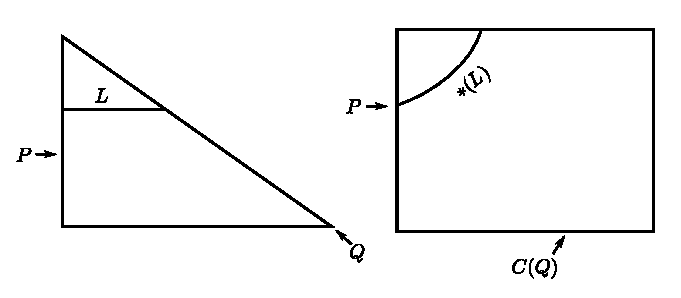
\includegraphics{figure/fig9.eps}
\end{figure}

The horizontal line segment corresponds to the part of a hyperbola under the above correspondence.
\end{example*}

We can however find a polyhedral substitute for this homeomorphism.

\setcounter{proposition}{7}
\begin{proposition}\label{chap4-prop4.3.8}
Let $P$, $Q$, $\alpha$, $\beta$ be as above, let $0<\tau<1$. Then there is a polyhedral equivalence.
$$
\mathcal{L}^{-1}([0,\tau])\approx P\times \beta^{-1}([0,\tau])
$$
which is consistant with the projection onto the interval $[0,\tau]$.
\end{proposition}

\begin{proof}
Let $\mathscr{P}$ and $\mathcal{Q}$ be simplicial presentations of $P$ and $Q$ and take the simplicial presentation $\mathscr{T}=\{\{0\},\{\tau\},(0,\tau)\}$ of $[0,\tau]$.

Consider\pageoriginale the set of all sets of the form $A(\rho,\sigma,i)$, where $\rho\in \mathscr{P}$, $\sigma\in\mathcal{Q}$, $i\in\mathscr{T}$ and $\sigma=\emptyset$ iff $i=\{0\}$, defined thus:
\begin{align*}
& A(\rho,\emptyset,0)=\rho\\
& A(\rho,\sigma,i)=\rho \sigma\cap \mathcal{L}^{-1}(i)
\end{align*}

The set of all these $A(\rho,\sigma,i)$, call it $\mathfrak{a}$. It is claimed that $\mathfrak{a}$ is a regular presentation of $\mathcal{L}^{-1}([0,\tau])$, and that $A(\rho,\sigma,i)\leq A(\rho',\sigma',i')$ if and only if $\rho\leq \rho'$, $\sigma\leq \sigma'$, $i\leq i'$. 

Secondly, consider the set of all sets of the form $B(\rho,\sigma,i)$ where $\rho\in \\mathscr{P}$, $\sigma\in\mathcal{Q}$, $i\in\mathscr{T}$, and $\sigma=\emptyset$ if $i=\{0\}$ defined thus:
\begin{align*}
& B(\rho,\emptyset,0)=\rho\times\{v\}\\
& B(\rho,\sigma,i)=\rho\times(\sigma\{v\}\cap \beta^{-1}(i))
\end{align*}

It is claimed that $\mathscr{B}$ of all such $B(\rho,\sigma,i)$ is a regular presentation of $P\times \mathscr{B}^{-1}([0,\tau])$, and that $B(\rho,\sigma,i)\leq B(\rho',\sigma',i')$ if and only if $\sigma\leq \sigma'$, $\rho\leq \rho'$ and $i\leq i'$.

Hence the correspondence $A(\rho,\sigma,i)\leftrightarrow B(\rho,\sigma,i)$ is a combinatorial equivalence $\mathfrak{a}\leftrightarrow\mathscr{B}$. If we choose the centerings $\eta$ and $\mathscr{V}$ of $\mathfrak{a}$ and $\mathscr{B}$ respectively such that
$$
\mathcal{L} (\eta(A(\rho,\sigma,(0,\tau)))=\tau/2
$$
and $\beta$ (2 nd coordinate of $\mathscr{V}(B(\rho,\sigma,(0,\tau)))=\tau/2$. The induced simplicial isomorphism $d(\mathfrak{a},\eta)\leftrightarrow d(\mathscr{B},\mathscr{V})$ gives a polyhedral equivalence $\mathcal{L}^{-1}([0,\tau)]\approx P\times \mathscr{B}^{-1}([0,\tau])$, consistent with the projection onto $[0,\tau]$. 

It should perhaps be remarked that by choosing $\mathscr{P}$ and $\mathcal{Q}$ fine\pageoriginale\break enough, our equivalence is arbitrarily close to the correspondence (*) on page 67.
\end{proof}

\begin{corollary}\label{chap4-coro4.3.9}
Let $C(P)$ be the cone on $P$ with vertex $v$, and $\mathcal{L}:C(P)\to [0,1]$ be the join of $P\to 0$, $v\to 1$. Then for any $\tau\in (0,1)$, $\mathcal{L}^{-1}([0,\tau])$ is polyhedrally equivalent to $P\times [0,\tau]$ by an equivalence consistent with the projection to $[0,\tau]$.  

For, take $Q=v$ in \ref{chap4-prop4.3.8}.
\end{corollary}

\begin{corollary}\label{chap4-coro4.3.10}
Let $\mathcal{L}:P\ast Q\to [0,1]$ be the join of $P\to 0$, $Q\to 1$; let $0<\gamma<\delta< 1$. Then $\mathcal{L}^{-1}([\gamma,\delta])$ is polyhedrally equivalent to $P\times Q\times[\gamma,\delta]$ by an equivalence consistent with the projection to $[\gamma,\delta]$.

For, by \ref{chap4-prop4.3.8}, $\mathcal{L}^{-1}([0,\delta])\approx P\times \beta^{-1}([0,\delta])$ where $\beta:C(Q)\to [0,1]$ is the join of $Q\to 1$ and vertex $\to 0$. By \ref{chap4-coro4.3.9}, interchanging $0$ and $1$, we see that $\beta^{-1}([\gamma,1]\approx Q\times [\gamma,1]$; combining these and noting the preservation of projection on $[\gamma,\delta]$, we have the desired result.
\end{corollary}

\begin{definition}\label{chap4-defi4.3.11}
Let $K$ be a polyhedron and $x\in K$. Then a subpolyhedron $L$ of $K$ is a said to be a (polyhedral) {\em link} of $x$ in $K$, if $L\ast x$ is defined, is contained in $K$, and is a neighbourhood of $x$ in $K$.
\end{definition}

A (polyhedral) {\em star} of $x$ in $K$ is the cone with vertex $x$ on any link of $x$ in $K$.

Clearly, if $a\in K_{1}\subset K$, and $K_{1}$ is a neighbourhood of `$a$' in $K$, then $L\subset K_{1}$ is a link of `$a$' in $K_{1}$, if and only if it is a link of `$a$' in $K$.

To\pageoriginale show that links and stars exist, we triangulate $K$ by a simplicial presentation $\mathscr{S}$ with $x$ as a vertex. Then $|Lk(x,\mathscr{S})|$ is a link of $x$ in $K$, and $|St(x,\mathscr{S})|$ is a star of $x$ in $K$. In this case $|St(x,\mathscr{S})|-|Lk(x,\mathscr{S})|$ is open in $K$; this need not be true for general links and stars.

\begin{ex}\label{chap4-ex4.3.12}
If $\mathscr{S}$ is any simplicial presentation of $K$, and $x\in \sigma\in\mathscr{S}$, then $|\{\p \sigma\}\ast Lk(\sigma,\mathscr{S})|$ is a link of $x$ in $K$, and $|\{\overline{\sigma}\}\ast Lk(\sigma,\mathscr{S})|$ is a star of $x$ in $K$.

(b)~ With $\delta A$, $\lambda A$ as in \ref{chap4-defi4.2.1}, if $x\in A$, $\p A\ast |\lambda A|$ is a link of $x$ in $K$. 
\end{ex}

\setcounter{proposition}{11}
\begin{dashex}\label{chap4-dashex4.3.12'}
\begin{itemize}
\item[(a)] Let $f:K\to K'$ be a one-to-one polyhedral map, simplicial with reference to presentations $\mathscr{S}$ and $\mathscr{S}'$ of $K$ and $K'$. Then for any $\sigma\in \mathscr{S}$, $x\in \sigma$
\begin{align*}
& f||\{\overline{\sigma}\}\ast Lk(\sigma,\mathscr{S})|\quad \text{is the join of}\\
& f||\{\p \sigma\}\ast Lk(\sigma,\mathscr{S})|\quad\text{and~ } x\to f(x).
\end{align*}

Formulate and prove a more general statement using \ref{chap4-ex4.1.16}

\item[(b)] With the hypothesis of \ref{chap4-ex4.2.15}, if $A_{0}$ is a $0$-cell of $\mathscr{P}$, $f(|\lambda A_{0}|)\subset |\lambda (fA_{0})|$ and
$$
f||\delta A_{0}|\quad\text{is the join of}\quad A_{0}\to f(A_{0})\quad\text{and}\quad f||\lambda A_{0}|.
$$
\end{itemize}
\end{dashex}

If $x$ and $a$ are two distinct points in a vector space, the set of points $(1-t)x+ta$, $t>0$  will be called `{\em the ray from $x$ through $a$}'.

Let $L_{1}$ and $L_{2}$ be two links of $x$ in $k$, then for each point $a\in L_{1}$, the ray through $a$ from $x$ intersects $L_{2}$ in a unique point $h(a)$ (and every point in $L_{2}$ is such a image). It intersects\pageoriginale $L_{2}$ in atmost one point, since the cone on $L_{2}$ with vertex $x$ exists. It intersects $L_{2}$ in at least one point since the cone on $L_{2}$ must contain a neighbourhood of the vertex of the cone on $L_{1}$.

The function $h:L_{1}\to L_{2}$ thus defined is a homeomorphism. But, perhaps contrary to intution, it is {\em not} polyhedral.
\begin{figure}[H]
\centering

\includegraphics{figure/fig10.eps}
\end{figure}

The graph of the map $h$ in this simple case is a segement of a hyperbola.

The fallacy of believing $h$ is polyhedral is old (See, Alexander ``The combinatorial theory of complexes'', Annals of Mathematics, 31, 1930); for this reason we shall call $h$ the {\em standard mistake} after Zeeman (see Chapter I of ``Seminar on Combinatorial Topology''). We shall show how to approximate it very well by polyhedral equivalences.

It might be remarked that the standard mistake is ``piecewise projective'', the category of such maps has been studies by N.H.\@ Kuiper [see ``on the Smoothings of Triangulated and combinatorial Manifolds'' in ``Differential and combinatorial Topology'', A symposium in Honor of Marston Morse, Edited by S.S.\@ Cairns].

\begin{definition}\label{chap4-defi4.3.13}
Let $A$ and $B$ be two convex sets. A one-to-one function from $A$ onto $B$, $\mathcal{L}:A\to B$ is said to be {\em quasi-linear}; if for each $a_{1}$, $a_{2}\in A$, $\mathcal{L}([a_{1},a_{2}])=[\mathcal{L}(a_{1}), \mathcal{L}(a_{2})]$.
\end{definition}

In other words, $\mathcal{L}$ preserves line segments. It is easy to\pageoriginale see that $\mathcal{L}^{-1}$ is also quasi-linear.

\begin{example*}
Any homeomorphism of an interval is quasi-linear. In $\mathbb{R}^{2}$, the map: 
$$
(r_{1},r_{2})\to \left(\frac{r_{1}}{1-r_{1}},\frac{r_{2}}{1-r_{1}}\right)
$$
as a map from $A=\{(r_{1},r_{2})\mid 0<r_{i}<1\}$ to $B=\{(\mathscr{S}_{1},\mathscr{S}_{2})\mid \mathscr{D}>\mathscr{S}_{i}>0\}$ is quasi-linear.
\end{example*}

\begin{proposition}\label{chap4-prop4.3.14}
Let $\mathcal{L}:A\to B$ be quasi-linear. Let $\{a_{0},\ldots,a_{n}\}$ be an independent set of points in $A$, defining an open simplex $\sigma$. Then $\{\mathcal{L}(a_{0}),\ldots, \mathcal{L}(a_{n})\}$ is independent, and the simplex they define is $\mathcal{L}(\sigma)$. Consequently $\tau$ is a face of $\sigma$ if and only if $\mathcal{L}(\tau)$ is a face of $\mathcal{L}(\sigma)$.
\end{proposition}

The proof is by induction. For $n=1$, this is the definition. The inductive step follows by writing $\sigma=\sigma'\{a_{n}\}$ and noting that quasi-linear map preserves joins.

\begin{theorem}\label{chap4-thm4.3.15}
Let $L_{1}$ and $L_{2}$ be two links of $x$ in $K$ with $h:L_{1}\to L_{2}$, the standard mistake. Suppose $\mathscr{Z}_{1}$ and $\mathscr{Z}_{2}$ are polyhedral presentations of $L_{1}$ and $L_{2}$. Then there exist simplicial refinements $\mathscr{S}_{1}$ and $\mathscr{S}_{2}$ of $\mathscr{Z}_{1}$ and $\mathscr{Z}_{2}$ such that for each $\sigma\in \mathscr{S}_{1}$, $h(\sigma)\in \mathscr{S}_{2}$ and $h|\overline{\sigma}$ is quasi-linear. If $f:L_{1}\to L_{2}$ is defined as the linear extension of $h$ restricted to the vertices of $\mathscr{S}_{1}$, then $f$ is a polyhedral equivalence simplicial with respect to $\mathscr{S}_{1}$ and $\mathscr{S}_{2}$ and such that $f(\sigma)=h(\sigma)$ for all $\sigma\in \mathscr{S}$ .
\end{theorem}

\begin{proof}
We can suppose that $\mathscr{Z}_{1}$ and $\mathscr{Z}_{2}$ are simplicial, and find a\pageoriginale simplicial presentation $\mathscr{P}$ of $(L_{1}\ast x\cup L_{2}\ast x)$ refining $(\mathscr{Z}_{1}\ast\{\{x\}\}\cup \mathscr{Z}_{2}\ast\{\{x\}\})$. Define $\mathscr{S}=Lk(x,\mathscr{P})$. It is clear that every simplex $\sigma\in \mathscr{S}$ is contained in $\tau\ast\{x\}$, for $\tau\in \mathscr{Z}_{1}$, and hence the standard mistake $h_{1}:|\mathscr{S}|\to L_{1}$ takes $\overline{\sigma}$ to $h_{1}(\overline{\sigma})\subset \overline{\tau}$.

The restriction of $h_{1}$ to $\overline{\sigma}$ is quasi-linear. For, let $a_{1}$, $a_{2}\in\overline{\sigma}$; the three points $a_{1}$, $a_{2}$, $x$ determine a plane and in that plane an angular region $L$, which is the union of all rays from $x$ through the points of $[a_{1},a_{2}]$. The standard mistake, by definition, takes $[a_{1},a_{2}]\subset\overline{\sigma}$ to $L\cap \overline{\tau}$, which, it is geometrically obvious, is just $[h_{1}(a_{1}), h_{1}(a_{2})]$.

This, together with \ref{chap4-prop4.3.14}, enables us to define $\mathscr{S}_{1}=\{h_{1}(\sigma)\mid \sigma\in\mathscr{S}\}$, and to see that this is a simplicial presentation refining $\mathscr{Z}_{1}$.

Similarly, via the standard mistake $h_{2}:|\mathscr{S}|\to L_{2}$, we have
$$
\mathscr{S}_{2}:\{h_{2}(\sigma)\mid \sigma \in \mathscr{S}\}.
$$

Since, clearly, $h:L_{1}\to L_{2}$ is $h_{2}  \circ h^{-1}_{1}$ and the composition and inverse of quasi-linear maps are again quasi-linear, the major part of the theorem is proved.

The last remark about $f$ is obvious.
\end{proof}

\setcounter{subsection}{15}
\subsection{}\label{chap4-sec4.3.16}
If in \ref{chap4-thm4.3.15}, for a subpolyhedron $K'$ of $L_{1}$, $h|K'$ is polyhedral, then we can arrange for $f:L_{1}\to L_{2}$ of the theorem to be such that $f|K'=h|K'$.

For, all we need to do is to assure that $\mathscr{Z}_{1}$ has a subpresentation\pageoriginale covering $K$; then because $h$ is linear on each simplex in $K$, the resultant $f$ is identical with $h$ there.

\setcounter{proposition}{16}
\begin{corollary}\label{chap4-coro4.3.17}
Links (resp.\@ stars) of $x$ in $K$ exist and all are all polyhedrally equivalent. 
\end{corollary}

\begin{proposition}\label{chap4-prop4.3.18}
If $f:P\to Q$ is a polyhedral equivalence, then any link of $x$ in $P$ is polyhedrally equivalent to any link of $x$ in $Q$.

For triangulate $f$, and look at the simplicial links; they are obviously isomorphic.
\end{proposition}

\medskip
\noindent{\textbf{4.3.18$^1$.}}
Allows to define the {\em local dimension} of {\em polyhedron $K$ at $x$.} This is defined to be the dimension of any star of $x$ in $K$. By \ref{chap4-coro4.3.17} this is well defined. It can be easily seen that (by \ref{chap4-ex4.3.12}) the closure of the set of points where the local dimension is $p$ is a subpolyhedron of $K$, for any integer $p$.

We will next consider links and stars in products and joins.

\begin{ex}\label{chap4-ex4.3.19}
Let $C(P)$ and $C(Q)$ be cones with vertices $v$ and $w$. Let $Z=(P\times C(Q))\cup (C(P)\times Q)$. Then 
\begin{itemize}
\item[(a)] $C(P)\times C(Q)=C(Z)$, the cone on $Z$ with vertex $(v,w)$

\item[(b)] $P\times w$ and $v\times Q$ are joinable, and $(P\times w)\ast (v\times Q)$ is a link of $(v,w)$ in $C(Z)$.
\end{itemize}

Hence by straightening our the standard mistake, we get a polyhedral equivalence $P\ast Q\approx Z$, which extends the canonical maps $P\to P\times w$ and\pageoriginale $Q\to v\times Q$.
\end{ex}

\noindent
{\bf Hint:}~It is enough to look at the following $2$-dimensional picture for arbitrary $p\in P$, $q\in Q$:
\begin{figure}[H]
\centering
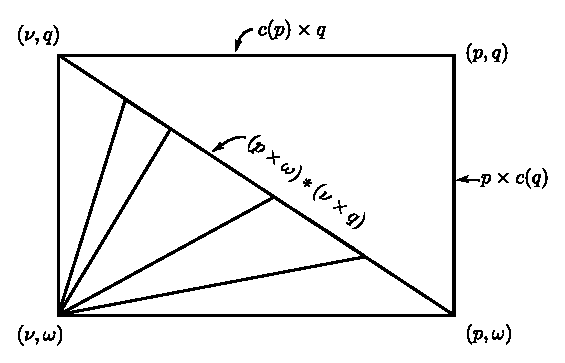
\includegraphics{figure/fig11.eps}
\end{figure}

\begin{ex}\label{chap4-ex4.3.20}
Prove that $P\ast Q\approx (C(p)\times Q\cup P\times C(Q))$ utilising \ref{chap4-prop4.3.8}. If $\varphi:P\ast Q\to [0,1]$ is the join of $P\to 0$, $Q\to 1$, the equivalence can be chosen so that $\varphi^{-1}([0,1/2])$ goes to $P\times C(Q)$ and $\varphi^{-1}([1/2,1])$ goes to $C(P)\times Q$.
\end{ex}

\begin{ex}[Links in products]\label{chap4-ex4.3.21}
If $x\in P$, $y\in Q$, then a link of $(x,y)$ in $P\times Q$ is the join of a link of $x$ in $P$ and a link of $y$ in $Q$.
\end{ex}

The join of $X$ to a polyhedron $\{x_{1},x_{2}\}$ consisting of two points is called {\em the suspension} of $X$ with {\em vertices} $x_{1}$ and $x_{2}$ and is denoted by $S(X)$. Similarly $K^{\text{th}}$ order suspensions are defined.

\begin{ex}[Links in joins]\label{chap4-ex4.3.22}
In $P\ast Q$.
\begin{enumerate}
\renewcommand{\labelenumi}{(\theenumi)}
\item  Let\pageoriginale $x\in P\ast Q-(P\cup Q)$, and let $x=(1-t)p+tq$, $p\in P$, $q\in Q$, $0<t<1$. If $L_{1}$ is a link of $p$ in $P$, $L_{2}$ a link of $q$ in $Q$, then $S(L_{1}\ast L_{2})$ (with vertices $p$, $q$) is a link of $x$ in $P\ast Q$.

\item If $p\in P$, and $L$ is a link of $p$ in $P$, then $L\ast Q$ is a link of $p$ in $P\ast Q$.
\end{enumerate}
\end{ex}

\noindent
{\bf Hint: for 1.}~ Consider simplicial presentations $\mathscr{P}$
and $\mathcal{Q}$ of $P$ and $Q$ having $p$ and $q$ as vertices. Then $Lk(p,\mathscr{P})\ast Lk(q,\mathcal{Q})$ is a link of $O(p,q)$ in $\mathscr{P}\ast \mathcal{Q}$, by \ref{chap4-ex4.1.11}. Hence a link of $x$ in $P\ast Q=|\{p,q\}\ast Lk(p,\mathscr{P})\ast Lk(q,\mathcal{Q})|$ or the suspension of $Lk(p,\mathscr{P})\ast Lk(q,\mathcal{Q})$ with vertices $p$ and $q$. The general case follows from this.

\section{Polyhedral cells, spheres and Manifolds}\label{chap4-sec4.4}

In this section, we utilize links and stars to define polyhedral cells, spheres and manifolds and discuss their elementary properties.

Let us go back to the open and closed (convex) cells discussed in \ref{chap1-sec1.5}. If $A$ is an open cell, then the closed cell $\overline{A}$ is the cone over $\p A$ with vertex $a$, for any $a\in A$.

\begin{proposition}\label{chap4-prop4.4.1}
If $A$ and $B$ are two open cells of the same dimension, then $\p A$ and $\p B$ are polyhedrally equivalent. Moreover the equivalence can be chosen to map any given point $x$ of $\p A$ onto any given point $y$ of $\p B$.
\end{proposition}

\begin{proof}
Let $\dim A=n=\dim B=n$. Via, a linear isomorphism of the linear manifolds containing $A$ and $B$, we can assume that $A$ and\pageoriginale $B$ are in the same $n$-dimensional linear manifold, and moreover that $A\cap B\neq \emptyset$. Then $\p A$ and $\p B$ are both links of any point of $A\cap B$ in $\overline{A}\cup \overline{B}$. Hence $\p A$ and $\p B$ are polyhedrally equivalent. A rotation of $A$ will arrange for the standard mistake to map $x$ to $y$. And \ref{chap4-thm4.3.15}, we can clearly arrange for $x$ and $y$ to be vertices in $\mathscr{S}_{1}$ and $\mathscr{S}_{2}$.
\end{proof}

By joining the above map with a map of point of $A$ to a point of $B$, we can extend it to a polyhedral equivalence of $\overline{A}$ and $\overline{B}$. Thus any two closed cells are polyhedrally equivalent.

\begin{definition}\label{chap4-defi4.4.2}
A {\em polyhedral $n$-sphere} (or briefly an {\em $n$-sphere}) is any polyhedron, polyhedrally equivalent to the boundary of an open cell of dimension $(n+1)$.
\end{definition}

By \ref{chap4-prop4.4.1} this is well defined.

\begin{definition}\label{chap4-defi4.4.3}
A {\em polyhedral $n$-cell} (or briefly an {\em $n$-cell}) is any polyhedron, polyhedrally equivalent to a closed convex cell of dimension $n$.
\end{definition}

By the remark after \ref{chap4-prop4.4.1}, this is well defined. All the cells and spheres except the $0$-sphere are connected.

Consider the ``standard $n$-cell'', the closed $n$-simplex, and the ``standard $(n-1)$-sphere'', the boundary of a $n$-simplex. By \ref{chap4-ex4.1.8}, \ref{chap4-prop4.3.18} and \ref{chap4-prop4.4.1}, we have

\begin{proposition}\label{chap4-prop4.4.4}
The link of any point in an $n$-sphere is an $(n-1)$-sphere.
\end{proposition}

\begin{corollary}\label{chap4-coro4.4.5}
An $n$-sphere is not polyhedrally equivalent to an $(m)$-sphere, if $m\neq n$. 
\end{corollary}

\begin{proof}
By\pageoriginale looking at the links using \ref{chap4-prop4.4.4}, and induction.
\end{proof}

\setcounter{subsection}{5}
\subsection{}\label{chap4-sec4.4.6}
If $f:D\approx \overline{\sigma}$ is an equivalence of an $n$-cell with a closed $n$-simplex $\overline{\sigma}$, we see that for points of $C$ corresponding to points of $\p \sigma$, the link in $C$ is an $(n-1)$-cell; and for points of $C$ corresponding to points of $\sigma$, the link in $C$ is an $(n-1)$-sphere.

\setcounter{proposition}{6}
\begin{proposition}\label{chap4-prop4.4.7}
An $n$-sphere is not polyhedrally equivalent to an $n$-cell.
\end{proposition}

\begin{proof}
Again by induction. For $n=0$, a sphere has two points and a cell has only one point.

For $n>0$, an $n$-cell has points which have $(n-1)$-cells as links, where as in a sphere all points have $(n-1)$-spheres as links. And so, by induction on $n$ they are different.
\end{proof}

This allows us to define boundary for arbitrary $n$-cells, namely the boundary of an $n$-cell $C$, is the set of all points of $C$ whose links are $(n-1)$-cells. We will denote this also by $\p C$. This coincides with the earlier definition for the boundary of a closed convex cell, and the boundary of a $n$-cell is an $(n-1)$-sphere. And as in \ref{chap4-coro4.4.5}, an $n$-cell and an $(m)$-cell are not polyhedrally equivalent if $m\neq n$.

By taking a particularly convenient pairs of cells and sphere, the following proposition is easily proved:

\begin{ex}\label{chap4-ex4.4.8}
Whenever they are defined,
\begin{enumerate}
\renewcommand{\labelenumi}{(\theenumi)}
\item The join a $m$-cell and an $n$-cell is a $(m+n+1)$-cell.

\item The join of a $m$-cell and an $n$-sphere is a $(m+n+1)$-cell.

\item The\pageoriginale join of a $m$-sphere and an $n$-sphere is a $(m+n+1)$-sphere.
\end{enumerate}

If in (1) of \ref{chap4-ex4.4.8}, $C_{1}$ and $C_{2}$ are the cells, then $\p (C_{1}\ast C_{2})=\p C_{1}\ast C_{2}\cup C_{1}\ast \p C_{2}$. In (2) of \ref{chap4-ex4.4.8}, if $C$ is the cell, and $S$ the sphere $\p (C\ast S)=\p C\ast S$.
\end{ex}

\begin{definition}\label{chap4-defi4.4.9}
A {\em PL-manifold of dimension $n$} (or a $PL$ $n$-manifold) is a polyhedron $M$ such that for all points $x\in M$, the link of $x$ in $M$ is either an $(n-1)$-cell or an $(n-1)$-sphere.
\end{definition}

\begin{definition}\label{chap4-defi4.4.10}
If $M$ is a PL $n$-manifold, then the boundary of $M$ denoted by $\p M$, defined to be $\p M=\{x\in M\mid \text{ link of $x$ in $M$ is a cell}\}$.
\end{definition}

\begin{notation*}
If $A$ is any subset of $M$, the interior of $A$ and the boundary of $A$ in the topology of $M$, will be denoted by int ${}_{M}A$ and bd ${}_{M}A$ respectively. $M-\p M$ is also usually called the interior of $M$, this we will denote by int $M$ or $\overset{\circ}{M}$. Note that $\text{int}_{M}M=M$, where as int $M=M-\p M$.

It is clear from the proposition above, the manifolds of different dimensions cannot be polyhedrally equivalent, of course, from Brouwer's theorem on the ``Invariance of domain'', it follows that they cannot even be homeomorphic.
\end{notation*}

\begin{proposition}\label{chap4-prop4.4.11}
If $M$ is a PL $n$-manifold, then $\p M$ is a PL $(n-1)$-manifold, and $\p(\p M)=\emptyset$.
\end{proposition}

\begin{proof}
We first observe that $M-\p M$ is open in $M$. For if $x\in M-\p M$, let $L$ be a link of $x$ in $M$, $S$ the corresponding star, such that $S-L$ is open in $M$. $S$ is a cell and $\p S=L$. If\pageoriginale $y\in S-L$, then a link of $y$ in $S$ is a link of $y$ in $M$, since $S$ is a neighbourhood of $y$. Since $S$ is a cell and $y\in S-\p S$, the link of $y$ in $S$ is a sphere. Hence $y\in M-\p M$, for all $y\in S-L$ or $M-\p M$ is open in $M$. Hence $\p M$ is closed in $M$. 

If $\mathscr{S}$ is any simplicial presentation of $M$ and $\sigma\in \mathscr{S}$, the $|\{\p \sigma\}\ast Lk(\sigma,\mathscr{S})\}$ is a link of $x$ in $M$ for all $x\in \sigma$ by \ref{chap4-ex4.3.12}. Hence $\sigma\subset \p M$ or $\sigma\subset M-\p M$. If $\sigma\subset \p M$, $\p \sigma$ also is contained in $\p M$, since $\p M$ is closed. $\p M$ being the union of all such $\overline{\sigma}$ is a subpolyhedron of $M$.

Let $x$ be a point of $\p M$, $L$ a link of $x$ in $M$ and $S=L\ast x$, the corresponding star such that $S-L$ is open. $L$ is an $(n-1)$-cell. And by \ref{chap4-ex4.4.8}, $S$ is an $n$-cell with $\p S=L\cup x\ast \p L$. If $y\in x\ast \p L-\p L\subset S-L$, then a link of $y$ in $S$ is a link of $y$ in $M$ as above. But a link of $y$ in $S$ is a cell, since $y\in \p S$. Hence $x\ast \p L-\p L\subset \p M$. Since $\p M$ is closed, $x\ast\p L\subset \p M$, and since $x\ast\p L$ is a neighbourhood of $x$ in $\p M$, $\p L$ is a link of $x$ in $\p M$. Hence $\p M$ is a PL $(n-1)$-manifold without boundary.
\end{proof}

\begin{remark*}
Thus, if $x\in \p M$, there exist links $L$ of $x$ in $M$ (for example, the links obtained using simplicial presentations), such that $\p L\subset \p M$ and $\p L$ a link of $x$ in $\p M$. This need notbe true for arbitrary links. Also there exists links $L$ of $x\in \p M$ in $M$, such that $L\cap \p M=\p L$. For example, take a regular presentation $\mathscr{P}$ of $M$ in which $x$ is a vertex and take $|\delta_{\mathscr{P}}\{x\}|$.
\end{remark*}

\begin{proposition}\label{chap4-prop4.4.12}
Let\pageoriginale $M$ be a PL $n$-manifold, and $\mathscr{S}$ a simplicial presentation of $M$. If $\sigma\in\mathscr{S}$, then either $\sigma\subset \p M$ or $M-\p M$, and
\begin{itemize}
\item[\rm(1)] $|Lk(\sigma,\mathscr{S})|$ is a $(n-k-1)$-cell if $\sigma\subset \p M$ 

\item[\rm(2)] $|Lk(\sigma,\mathscr{S})|$ is a $(n-k-1)$-sphere if $\sigma\subset M-\p M$ where $k$ is the dimension of $\sigma$.
\end{itemize}
\end{proposition}

\begin{proof}
That $\sigma\subset \p M$ or $M-\p M$ is proved in \ref{chap4-prop4.4.11}. The proof of (1) and (2) is by induction on $k$. It $k=0$, this follows from definition. If $k>0$, let $\tau$ be a $(k-1)$-face of $\sigma$. Then $Lk(\sigma,\mathscr{S})=Lk(\tau,\{\p\sigma\}\ast Lk(\sigma,\mathscr{S}))$, and $|\{\p \sigma\}\ast Lk(\sigma,\mathscr{S})|$ being the link of a point in $\sigma$ is either $(n-1)$-sphere or a $(n-1)$-cell. Hence, by induction, $Lk(\sigma,\mathscr{S})$ is either a cell or sphere of dimension $(n-1)-(k-1)-1=(n-k-1)$. If $\sigma\subset \p M$, $|\{\p \sigma\}*Lk(\sigma,\mathscr{S})|$ is a cell. Hence $|Lk(\sigma,\mathscr{S})|$ cannot be a sphere, since then $|\{\partial \sigma\}| \ast Lk (\sigma, \mathscr{s})| = \partial \sigma \ast | Lk (\sigma, \mathscr{s})|$ would be a sphere. Thus if $\sigma\subset \p M$, $|Lk(\sigma,\mathscr{S})|$ is a $(n-k-1)$-cell. Similarly if $\sigma\subset M-\p M$, $|Lk(\sigma,\mathscr{S})|$ is a $(n-k-1)$-sphere.
\end{proof}

\begin{ex}\label{chap4-ex4.4.13}
(1)~ Let $M$ be a $PL$ $m$-manifold, and $N$ a $PL$ $n$-manifold. Then $M\times N$ is a $PL$ $(m+n)$-manifold and $\p (M\times N)$ is the union of $\p M\times N$ and $M\times \p N$.
\smallskip

\noindent
{\bf Hint:~} Use, \ref{chap4-ex4.3.21} and \ref{chap4-ex4.4.8}.
\medskip

(2)~ If $M\ast N$ is defined, it is not a manifold except for the three cases of \ref{chap4-ex4.4.8}.
\smallskip

\medskip
\noindent
{\bf Hint:}~ Use \ref{chap4-ex4.3.22}.
\end{ex}

\begin{proposition}\label{chap4-prop4.4.14}
\begin{itemize}
\item[\rm(a)] If\pageoriginale $f:S\to S'$ is a one-to-one polyhedral map of an $n$-sphere $S$ into another $n$-sphere $S'$, then $f$ is onto.

\item[\rm(b)] If $f:C\to C'$ is a one-to-one polyhedral map of an $n$-cell $C$ into another $n$-cell $C'$ such that $f(\p C)\subset \p C'$, then $f$ is onto.
\end{itemize}
\end{proposition}

\noindent
{\bf Proof of (a):}~ By induction. If $n=0$, $S$ has two points and the proposition is trivial. Let $n>0$. Let $f$ be simplicial with respect to presentations $\mathscr{S}_{1}$ and $\mathscr{S}_{2}$ of $S$ and $S'$. If $x$ is any point of $S$, $x\in\sigma$ for some $\sigma\in \mathscr{S}_{1}$. Consider
\begin{align*}
L_{1} &= |\{\p \sigma\}\ast Lk(\sigma,\mathscr{S}_{1})|,\ S_{1}=|\{\p \overline{\sigma}\}\ast Lk(\sigma,\mathscr{S}_{1})|,\\
L_{2} &= |\{\p(f\sigma)\}\ast Lk(f\sigma,\mathscr{S}_{2})|,\ \text{ and }\ S_{2}=|\{f\overline{\sigma}\}\ast Lk(f\sigma,\mathscr{S}_{2})|. 
\end{align*}

Since $f$ is injective $f$ maps $L_{1}\to L_{2}$, and $f|S_{1}$ is the join of $f|L_{1}$ and $x\to f(x)$. $L_{1}$ and $L_{2}$ are $(n-1)$-spheres, and by induction $f|L_{1}$ is bijective. Therefore $f(S_{1})=S_{2}$. Hence $f(S)$ is open in $S'$. Since $S$ is compact $f(S)$ is closed in $S'$. Since $S$ is connected, $f(S)=S'$. (b) is proved similarly.

By the same method, it can be shown

\begin{ex}\label{chap4-ex4.4.15}
There is no one-to-one polyhedral map of an $n$-sphere into an $n$-cell.
\end{ex}

\begin{ex}\label{chap4-ex4.4.16}
\begin{enumerate}
\renewcommand{\labelenumi}{(\theenumi)}
\item A PL-manifold cannot be imbedded in another PL-manifold of lower dimension. 

\item If $M$ and $N$ are two connected manifolds of the same dimension, $\p N\neq \emptyset$, and $\p M=\emptyset$, then $M$ cannot be embedded in $N$. If $\p N$ is also empty, and if $M$ can be embedded in $N$ then $M\approx N$.
\end{enumerate}
\end{ex}

\begin{ex}\label{chap4-ex4.4.17}
\begin{enumerate}
\renewcommand{\labelenumi}{(\theenumi)}
\item If\pageoriginale $M\subset N$ are two $PL$ $n$-manifolds, then $M-\p M\subset N-\p N$, and $M-\p M$ is open in $N$.
\noindent
{\bf Hint:}~ Use \ref{chap4-prop4.4.14} and \ref{chap4-ex4.4.15}.

In particular any polyhedral equivalence of $N$ has to take $N-\p N$ onto $N-\p N$ and $\p N$ onto $\p N$.

\item If $M\subset N-\p N$, both $M$ and $N$, $PL$ $(n)$-manifolds, and $x$ any point of $\p M$, show that there exist links $L$ of $x$ in $N$, such that a link of $x$ in $M$ is an $(n-1)$-cell $D\subset L$, and $D\cap \p M=\p D$.
\end{enumerate}
\end{ex}

\begin{ex}\label{chap4-ex4.4.18}
In \ref{chap4-coro4.2.14}, show that if $P$ is a PL $n$-manifold $f^{-1}(q)(\p\neq \emptyset)$ is a PL $(n-m)$-manifold and $\p (f^{-1}(q))\subset \p P$.
\end{ex}

\section{Recalling Homotopy Facts}\label{chap4-sec4.5}

Here we discuss some of the homotopy facts needed later. The reader is referred to any standard book on homotopy theory for the proof of these.

\subsection{}\label{chap4-sec4.5.1}
We define a space $P$ to be {\em $(k-1)$-connected} iff, for any polyhedra $Y\subset X$, with $\dim X\leq k$, every continuous map $Y\to P$ has an extension to $X$.

Thus, a $(-1)$-connected polyhedron must just be non-empty. A $k$-connected polyhedron for $k\leq -2$, can be anything. For $k\geq 0$, it is necessary and sufficient that $P$ be non-empty and that $\pi_{i}(P)=0$ for $i\leq k$.

\subsection{}\label{chap4-sec4.5.2}
A pair of spaces $(A,B)$ where $B\subset A$, is {\em $k$-connected} if for any polyhedra $Y\subset X$ with $\dim X\leq k$, and $f:X\to A$ such that $f(Y)\subset B$, then $f$ is homotopic to a map $g$, leaving $Y$ fixed, such that $g(X)\subset B$.

This\pageoriginale is just the same as requiring that $\pi_{i}(A,B)=0$ for $i\leq k$. If $A$ is contractible (or just $(k-1)$-connected) and $(A,B)$ is $k$-connected, then $B$ is $(k-1)$-connected.

We shall have occasion to look at pairs of the form $(A,A-B)$, which we denoted briefly as $(A,-B)$. The following discussion is designed to suggest how to prove a result on the connectivity of joins, which is well known from homotopy theory. 

\subsection{}\label{chap4-sec4.5.3}
Let $A_{1}\subset A$, $B_{1}\subset B$, and suppose $(A,-A_{1})$ is $a$-connected, $(B,-B_{1})$ is $b$-connected. Then $(A\times B,-A_{1}\times B_{1})$ is $(a+b+1)$-connected.

Let $Y\subset X$, $\dim X\leq a+b+1$, and $f:X\to A\times B$, with $f(Y)\cap A_{1}\times B_{1}=\emptyset$.

We must now triangulate $X$ finely by say $\mathscr{S}$. Look at $|\mathscr{S}_{a}|=X_{1}$ and $|\mathscr{S}^{a+1}|=X_{2}$. Then $\dim X_{1}\leq a$, $\dim X_{2}\leq b$, and so the two coordinates of $f$ are homotopic, using homotopy extension, to get a map, still called $f_{1}$ such that
$$
f_{A}(X_{1})\cap A_{1}=\emptyset,\quad f_{B}(X_{2})\cap B_{1}=\emptyset.
$$

Because $X-X_{2}$ has $X_{1}$ as a deformation retract, we can first get $f_{B}(X_{2})\cap B_{1}=\emptyset$ and then $f^{-1}(A_{1}\times B_{1})$ is contained in $X-X_{2}$. By changing, homotopically, only the first coordinate, we get $f^{-1}(A_{1}\times B_{1})=\emptyset$.

To go more deeply into this sort of argument, see Blakers and\break Massey, ``Homotopy groups of Triads'' I, II, III'', Annals of Mathematics Vol.\@ 53, 55, 58.

\subsection{}\label{chap4-sec4.5.4}
If $P$ is $(a-1)$-connected, $Q$ is $(b-1)$-connected, then $P\ast Q$ is\pageoriginale $(a+b)$-connected.

For, let $C(P)$, $C(Q)$ be cones with vertices $v$, $w$. Then $(C(P),-v)$ is $a$-connected, $(C(Q),-w)$ is $b$-connected. Hence by \ref{chap4-sec4.5.3}, $(C(P)\times C(Q),-(v,w))$ is $(a+b+1)$-connected. By \ref{chap4-ex4.3.19}, this pair is equivalent to $(C(P\ast Q),-(v,w))$. Hence $P\ast Q$ is $(a+b)$-connected. For a direct proof of \ref{chap4-sec4.5.4}, see Milnor's ``Construction of Universal Bundles II (Annals of Mathematics, 1956, Vol.\@ 63).

\subsection{}\label{chap4-sec4.5.5}
The join of $K$ non-empty polyhedra is $(k-2)$-connected. In particular $(k-1)$-sphere is $(k-2)$-connected. The join of a $(k-1)$-sphere and a $a$-connected polyhedron is $(a+k)$-connected. Thus a $k^{\text{th}}$ suspension (same as the join with a $(k-1)$-sphere) of a connected polyhedron is at least $K$-connected.


